\documentclass[11pt]{article}
\usepackage[T1]{fontenc}
\usepackage[utf8]{inputenc}
\usepackage{graphicx}
\usepackage{minitoc}
\usepackage[french]{babel}
\usepackage[right=2.5cm, bottom=2.5cm,top=2.5cm, left=2.5cm]{geometry}
\title{\vspace{\fill} Interface et Multimédia \\ ~\textbf{IFT-215} \\~\\ Travail Pratique 3}
\author{Amandine Fouillet - 14 130 638 ~\\ Frank Chassing - 14 153 710 ~\\ Laurent Sénécal-Léonard - 14 143 484}
\date{\today \vspace{\fill}}

\begin{document}
\maketitle
\newpage \thispagestyle{empty}
\null
\newpage
\tableofcontents

\newpage
\section*{Introduction \markboth{INTRODUCTION}{}}
\addcontentsline{toc}{section}{Introduction}
Dans le rapport précédent, nous avons mis en avant l’exploration et l’analyse des différentes tâches que réalisent des étudiants à l’étranger et leurs parents afin d’assurer une communication plus ou moins complète.  Nous avons également étudié les différents utilisateurs et leurs environnements pour apporter le plus d’informations possible. Au cours de ce premier rapport, nous nous sommes aperçus qu’il n’existait aucun moyen ou application qui permettait une communication efficace et complète. Nous avons donc choisi d’implémenter une solution qui permet de regrouper tous les moyens de communication au sein d’une même application. ~\\

Dans ce compte-rendu, nous réalisons l’étape de conception globale de la méthode LUCID. Pour cela, nous décrirons dans un premier temps l’interface principale de notre application en soulignant les différents liens qui existent entre les fenêtres. Dans un second temps, nous expliquerons les différentes fonctionnalités que nous avons décidé de voir apparaître dans notre application, et nous détaillerons celles-ci grâce à de premières ébauches d’interfaces. Enfin, nous montrerons en conclusion comment notre interface met en valeur l’analyse de tâche du rapport précédent et comment elle répond aux critères de celle-ci.
\section{Représentation globale de l'interface}
Dans cette première partie, nous allons décrire les grandes lignes de l'interface ainsi que les liens entre les différentes fenêtres de l'application. Tous les éléments graphiques de l'interface qui sont décrits dans ce rapport seront représentés visuellement dans l'annexe de ce rapport. Les dessins de l'interface ont été réalisés avec un logiciel et représentent notre application dans sa version OSX. Cependant, l'application pourra également être réalisée sur Windows et les supports mobiles comme iOS et Android. 
\subsection{Identité graphique}
Nous avons choisi de donner le nom "Awaï" à notre application. Ce nom rappelle le mot anglais "Away" qui signifie "Loin" et qui se rapporte à l'idée d'éloignement des familles qui utiliseront l'application. Nous avons changé le "y" par un "ï" pour ne pas utiliser le mot original et laisser un peu de mystère quant à la signification du nom. ~\\

Pour le logo, nous avons choisi une icône d'avion. Simple à représenter, et pas trop encombrant, ce logo rappelle également la notion d'éloignement et de distance entre les utilisateurs.~\\

Pour donner une cohérence entre toutes les fenêtres de l'application nous avons choisi de créer une petite identité graphique. Pour ce faire, nous avons décidé de reprendre des formes elliptiques  sur les différentes pages et d'appliquer un code couleur pastel (Figure \ref{fig:codecouleur}).
\subsection{La fenêtre de connexion}
Lors de la première utilisation, juste après son installation, l'application se lancera sur une fenêtre de connexion (Figure \ref{fig:connexion})pour permettre à l'utilisateur de s'identifier et ainsi d'avoir accès à son espace personnel. Cette fenêtre comporte peu d'éléments mis à par le nom de l'application et son logo en haut au centre, trois boutons situés au milieu de la page : Connexion, Inscription et À Propos et enfin deux boutons iconiques en bas à gauche représentant les paramètres et l'aide.~\\ 

L'utilisateur pourra choisir de cliquer sur le bouton "Connexion" s'il est déjà inscrit à l'application, il rentrera alors ses identifiants et accédera à son espace. Au contraire, si c'est la première fois qu'il utilise l'application il sélectionnera "Inscription" et rentrera ses coordonnées pour se créer un compte. Enfin, il peut souhaiter en savoir plus sur l'application et aller explorer ce qui se trouve derrière le bouton "À Propos".  Les rôles des liens vers les paramètres et l'aide seront expliqués plus en détails dans la section \ref{par:aide}.

\subsection{Architecture de la fenêtre principale}
Sur la fenêtre principale  (Figure \ref{fig:principale}), comme sur la fenêtre de connexion, on retrouve en haut au centre le nom de l'application et son logo ainsi que les icônes de paramètres et d'aide en bas à gauche. Au centre on retrouve deux rangées de trois ellipses colorées qui contiennent les icônes des fonctionnalités de l'application. Sur la première rangée on retrouve la communication (section \ref{par:com}), les photos (section \ref{par:photos}) et le calendrier (section \ref{par:cal}) tandis que sur la seconde on retrouve le suivi des dépenses (section \ref{par:depenses}), la carte du monde (section \ref{par:carte}) et les contacts (section \ref{par:contact}). En dessous de chaque ellipse représentant une fonctionnalité, on trouve une courte description textuelle de la fonctionnalité pour aider la compréhension des utilisateurs qui ne sauraient pas ce que l'icône signifie.

\subsection{Lien entre les fenêtres}
Dès que l'on sélectionne une fonctionnalité en cliquant sur une des ellipses, on quitte la fenêtre principale. Le décor diffère en fonction de la fonctionnalité dans laquelle on se trouve mais afin que l'utilisateur ne soit pas perdu, nous avons conservé une base graphique (Figure \ref{fig:base}) que l'on retrouvera dans chaque fonctionnalité. En effet, sur chaque fenêtre on retrouvera en haut à gauche une icône de maison pour le retour à l'accueil, les six ellipses représentant les fonctionnalités de notre application alignées les unes en dessous des autres sur le côté gauche de la fenêtre et, enfin, les icônes d'aide et de paramètres côte à côte en bas à gauche.
En fonction de la fonctionnalité dans laquelle l'utilisateur se trouve, une des ellipses aura disparu et seule l'icône de la fonctionnalité restera visible. De plus, le titre, l'ellipse et l'icône de la fonctionnalité seront rappelés en haut de la fenêtre.~\\

Sur certaines fenêtres, celles des fonctionnalités photos, calendrier, dépenses et carte on retrouve une icône de partage en haut à gauche. Cette icône permet à l'utilisateur de sélectionner les amis à qui il veut partager cette fonctionnalité. En effet, il peut par exemple vouloir partager des choses différentes à ses parents qu'à ses amis. Cet outil lui permet de contrôler l'accès de ses amis à ses données personnelles. ~\\

Pour naviguer d'une fonctionnalité à une autre il suffit simplement de cliquer sur son icône dans la barre permanente de gauche. On change alors de décors pour atterrir dans la nouvelle fonctionnalité. Sur un ordinateur, pour les utilisateurs qui veulent garder plusieurs vues de l'application ouvertes il est également possible d'ouvrir d'autres fenêtres en sélectionnant l'option nouvelle fenêtre dans le menu de l'application.

\section{Description des fonctionnalités}
Dans un second temps, nous allons vous décrire les fonctionnalités que nous avons souhaité apporter à notre application. Celles-ci ont été définies suite au recueil des besoins des utilisateurs dans notre précédent rapport. Toutes les fonctionnalités ont été réparties dans six grandes catégories que nous détaillons ci-dessous : la communication, le partage de photos, l'emploi du temps, les dépenses, la carte du monde et enfin, les contacts. Pour finir, nous donnerons un aperçu du système d'aide et de la gestion des paramètres de l'application.
\subsection{La communication}\label{par:com}
	Tout d’abord, cette fonctionnalité regroupe trois moyens de communication différents : les appels audio, les appels vidéo et la messagerie instantanée. Ceux-ci seront au libres  choix des utilisateurs. Pour les communications par appels, le fonctionnement de notre application sera semblable à celui de l’application Skype. En d’autres termes, les utilisateurs devront se mettre d’accord sur la date et l’heure à laquelle ils veulent se contacter. Il sera possible d’envoyer des messages instantanés à d’autres contacts lors des appels  et il sera possible d'inviter davantage de contact lors des communications. Puis, lorsqu’un utilisateur reçoit une invitation pour amorcer une conversation audio ou audio et vidéo, une alerte surviendra sur l’interface du récepteur demandant si oui ou non celui-ci désire commencer cette discussion. ~\\
	
	Ensuite, l’interface de cette fonctionnalité se décrit par une liste contenant les conversations récentes. Le nom du contact et sa photo sont affichés pour chacune des discussions. De plus, pour chacun des contacts le dernier message instantané reçu ou envoyé apparaît. Pour tous les contacts présents dans la liste, il y a à la droite de chacun d’eux un bouton ayant un téléphone de dessiné dans celui-ci et un deuxième bouton où une caméra vidéo y est dessinée. Ainsi, pour commencer une conversation audio, l’utilisateur doit cliquer sur le bouton «téléphone» et pour amorcer une conversation audio et vidéo l’utilisateur doit cliquer sur le bouton «caméra vidéo». Finalement, pour écrire un message instantané l’émetteur devra double-cliquer sur le contact désiré.
\subsection{Le partage de photos}\label{par:photos}
Cette fonctionnalité permettra à l’utilisateur de partager des photos qu’il désire montrer à son entourage. Lorsque ce dernier prend des photos, il lui sera possible de les publier dans cette fonctionnalité. Il pourra classer ses photos selon l’évènement en question ou selon la date où la photo a été prise. Afin que son entourage puisse voir les photos enregistrées dans le répertoire de cette fonctionnalité, l’utilisateur devra sélectionner les photos et cliquer sur partager avec le ou les contacts désirés.~\\

Au niveau de l’interface,  chaque répertoire de photos se présente par une bulle munie d’une photo de l’évènement à l’intérieur et du nom de l’évènement situé à l’extérieur de la bulle. Pour ajouter un répertoire de photo, un bouton (+) se trouvera sur la barre de menu qui permettra de faire l’action. L’utilisateur pourra donner un nom qu’il a choisi ou simplement ne pas donner de nom ce qui affichera par défaut la date de prise de photos. Finalement, un bouton de partage se trouve sur la barre des menus permettant à l’utilisateur de partager ses photos sélectionnées avec ses contacts.
\subsection{L'emploi du temps}\label{par:cal}
Cette fonctionnalité permet à l’utilisateur d’afficher la gestion de son temps à son entourage. Les informations ajoutées en entrée seront enregistrées dans un calendrier où il sera possible de choisir précisément l’heure de l'événement. Par souci de confidentialité, l’utilisateur pourra choisir à son aise les informations qu'il désire partager avec des contacts en particulier.~\\

Concernant l’interface, par défaut celle-ci se présente avec un calendrier affichant le mois en cours et ses journées numérotées. Il est possible pour l’utilisateur de changer la disposition du calendrier selon un format année avec les douze mois ou encore dans un format hebdomadaire avec les sept jours de la semaines. Pour ajouter un événement dans le calendrier, l'utilisateur sélectionne une journée puis grâce à un double clic il peut créer son événement et renseigner l'heure et l'intitulé. Finalement, un bouton pour partager son emploi du temps avec ses amis se trouve en haut à gauche de la fenêtre.
\subsection{Le suivi des dépenses}\label{par:depenses}
Pour commencer, cette fonctionnalité permet à l’utilisateur de faire une gestion de ses économies selon plusieurs catégories de dépenses. En effet, la fonctionnalité propose des catégories telles que vêtement, transport, logement, sorties, nourriture, etc. Ensuite, l’utilisateur peut choisir le mois qu'il désire pour ajouter une donnée et il doit pour chaque entrée écrire une description, un prix et une catégorie pour la dépense. Il sera possible de partager les informations de cette fonctionnalité avec les contacts de son choix.~\\

Au niveau de l’interface, celle-ci est divisée en deux parties. La première contient toutes les entrées nécessaires pour ajouter une dépense au programme. En effet, il y a des formulaires pour entrer sans forme prédéfini la description, le montant et la catégorie de la dépense. Le montant cumulé total du mois se trouve dans cette section. Un diagramme circulaire se trouve en bas de la page. Celui-ci a comme objectif de donner un résumé global des types de dépenses faites par l’utilisateur. Finalement, le bouton de partage se trouve dans le  menu de la fonctionnalité.
\subsection{La carte du monde}\label{par:carte}
Cette fonctionnalité n'a pas été évoquée directement dans le TP2 mais nous avons voulu la rajouter de manière à ce que les personnes éloignées puissent continuer à se suivre à distance. En effet, cette carte du monde permettra à l'étudiant d'indiquer avec des punaises les endroits où il s'est rendu, les lieux qu'il a visités. De cette manière, ses parents, ses grands-parents pourront suivre son chemin et ses aventures à distance. ~\\

Au niveau de l'interface, cette fonctionnalité se présente simplement comme une carte du monde que l'on peut parcourir, zoomer et dézoomer. Grâce à un appui plus long sur une zone de la carte, l'utilisateur peut rajouter une "punaise" pour signaler à ses amis qu'il s'est rendu dans cet endroit. Il choisit la couleur de la punaise en fonction de la raison de sa visite (une punaise rouge pour le lieu d'habitation, une punaise bleue pour les lieux scolaires et une punaise verte pour les visites).
\subsection{Les contacts}\label{par:contact}
La fonctionnalité des contacts référenciera l’ensemble des contacts que l’utilisateur aura préalablement ajouté. Ces contacts seront triés par ordre alphabétique. L’utilisateur pourra scroller la page pour faire dérouler l’ensemble des contacts. Chaque contact sera accompagné d’une photo, et de cinq icônes de fonctionnalités. L'icône de communication permettra de commencer une conversation écrite, audio ou bien vidéo avec le contact. L’icône de photographie garantira un accès à l’album photo du contact si celui-ci nous l’a autorisé. L’icône de l’emploi du temps permettra d’avoir un aperçu sur le calendrier du contact et de voir les disponibilités de celui-ci. L’utilisateur pourra suivre le suivi des dépenses du contact par le biais de l’icône des dépenses si celui-ci lui autorise l’accès. L’icône de la carte du monde donnera les différents lieux que le contact veut partager avec l’utilisateur. Il est à noter qu’il sera possible dans les paramètres d’effectuer des modifications sur le contact, comme par exemple le changement de photo ou de pseudo. Il est bien évident que l'utilisateur pourra ajouter un contact quand il le souhaite par le biais de cette page.~\\

Cette interface donne un accès rapide à chaque information que chaque contact veut partager. C’est à partir d’ici que l’utilisateur prendra des nouvelles et s’informera de ses proches. Il lui suffira de cliquer sur une des icônes d’un contact pour avoir accès à l’information désirée.

\subsection{Les paramètres et l'aide en ligne}\label{par:aide}
Afin de pouvoir informer, aider et donner des informations à un utilisateur qui utiliserait l’application, nous avons choisi de placer un bouton d’aide dans le coin inférieur gauche de chaque fenêtre. Nous avons jugé l’application plutôt simple à apprendre, c’est pourquoi nous n’encombrerons pas l’application de bulles d’aide ou de textes explicatifs. Si l’utilisateur ne comprend pas une chose, il se dirigera instantanément vers ce bouton d’aide. En fonction de l’endroit et du sous-menu dans lequel l’utilisateur se trouve, le contenu de la rubrique d’aide changera. Par exemple dans la fenêtre principale, nous retrouverons une FAQ (foire à question) qui permettra d’expliquer les différentes fonctionnalités du menu, tandis que dans les fenêtres comme « Communication » ou « Contacts », la rubrique d’aide aura des explications beaucoup plus détaillés pour expliquer chaque fonction que l’on peut effectuer dans la fenêtre. Ils pourront également posséder une FAQ ou bien un formulaire permettant de poser une question aux créateurs de l’application si l’utilisateur n’a pas trouvé la réponse qu’il cherche.~\\

Le bouton d’aide en ligne sera accompagné d’un bouton permettant d’accéder aux paramètres de l’application. Tout comme le bouton d’aide, nous aurons un contenu dynamique qui changera en fonction de la fenêtre dans laquelle on se trouve. Dans l’interface principale, nous pourrons ainsi gérer les notifications, les différents éléments du compte de l’utilisateur, la langue, etc. Dans les autres fenêtres, nous retrouverons directement des paramètres liés aux fonctionnalités. Par exemple, dans les paramètres de la fenêtre des « Contacts », nous retrouverons les paramètres associés tels que la gestion et la modification des contacts.

\newpage
\section*{Conclusion \markboth{CONCLUSION}{}}
\addcontentsline{toc}{section}{Conclusion}
Par le biais de notre analyse des tâches, nous avons pu observer les différentes applications qui existent pour que des étudiants puissent communiquer de l’étranger avec leur famille. L’étude des utilisateurs et de leurs environnements respectifs nous ont permis de lister un certain nombre d’applications susceptibles d’être utilisés. Cependant, nous avons remarqué qu’il n’existait pas d’applications réunissant l’ensemble des fonctionnalités qu’a besoin un étudiant pour communiquer à l’étranger. C’est pourquoi, nous avons envisagé une solution regroupant toutes les fonctionnalités utiles à la communication et des fonctionnalités nouvelles comme le suivi des dépenses, le partage de l’emploi du temps ou la géolocalisation en temps réel. Nous avons jugé indispensable de pouvoir naviguer aisément entre les différentes fonctionnalités, et donc nous avons mis en place une interface adéquate permettant cette navigation en laissant à disposition un menu couvrant les différentes fonctions de notre application. Nous avons travaillé chaque interface de chaque fonctionnalité pour que les utilisateurs puissent l’utiliser le plus simplement possible. Nous voulons avant tout que les utilisateurs apprennent  à utiliser cette application rapidement et puissent communiquer et accéder à toutes les fonctionnalités de façon fluide. Il est à savoir que les ébauches d’interfaces présentées ne sont définitives et pourraient bien entendu être modifiées par la suite.

\newpage
\section*{Annexes \markboth{ANNEXES}{}}
\addcontentsline{toc}{section}{Annexes}
\begin{figure}[hbtp]
        \centering 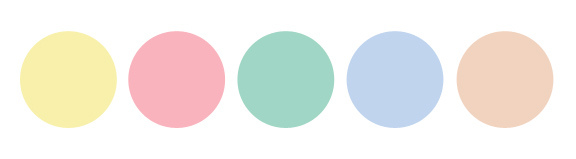
\includegraphics[scale=0.6]{Modelisation/Couleurs/pastels.jpg}
        \caption{Code couleur}
	\label{fig:codecouleur}
\end{figure}
\vspace{4cm}
\begin{figure}[hbtp]
    \begin{minipage}[b]{0.4\linewidth}
        \centering 
\includegraphics[scale=0.43]{Modelisation/connexion.png}
        \caption{Fenêtre de connexion}
	\label{fig:connexion}
    \end{minipage}\hfill
    \begin{minipage}[b]{0.48\linewidth}
        \centering 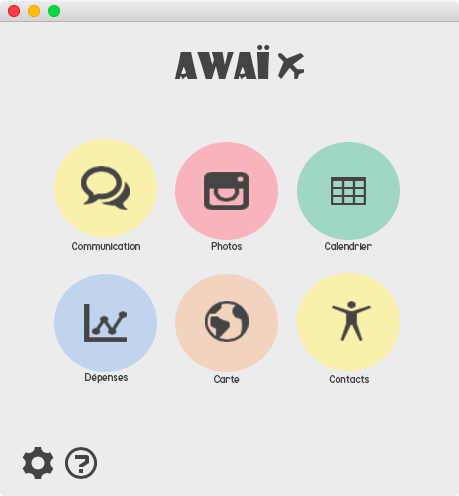
\includegraphics[scale=0.43]{Modelisation/awai.png}
       \caption{Fenêtre principale}
\label{fig:principale}
    \end{minipage}
\end{figure}
\begin{figure}[hbtp]
    \begin{minipage}[b]{0.4\linewidth}
        \centering 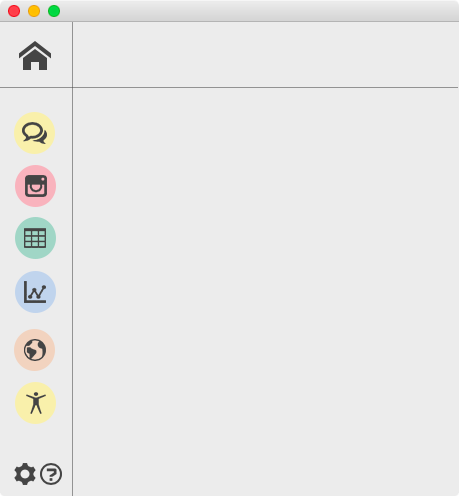
\includegraphics[scale=0.43]{Modelisation/base.png}
        \caption{Base de l'interface}
\label{fig:base}
    \end{minipage}\hfill
    \begin{minipage}[b]{0.48\linewidth}
        \centering 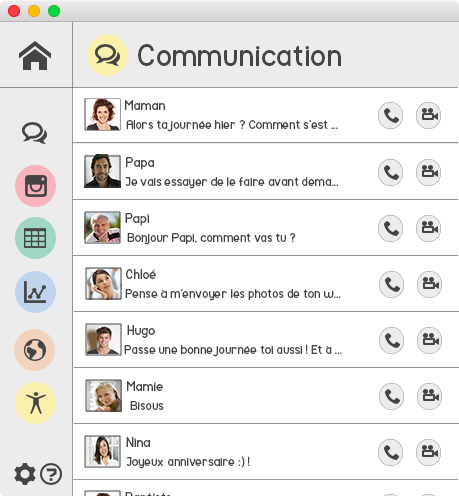
\includegraphics[scale=0.43]{Modelisation/communication.png}
        \caption{Gestion des communications}
        \label{fig:communication}
    \end{minipage}
\end{figure}
\begin{figure}[hbtp]
    \begin{minipage}[b]{0.4\linewidth}
        \centering 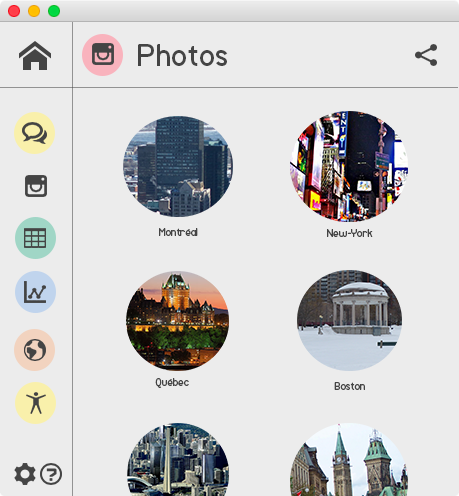
\includegraphics[scale=0.43]{Modelisation/photos.png}
        \caption{Gestion des photos}
                \label{fig:photos}
\label{fig:base}
    \end{minipage}\hfill
    \begin{minipage}[b]{0.48\linewidth}
        \centering 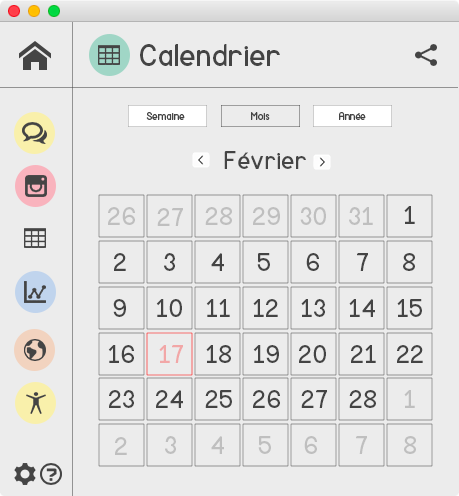
\includegraphics[scale=0.43]{Modelisation/calendrier.png}
        \caption{Gestion du calendrier}
        \label{fig:calendrier1}
    \end{minipage}
\end{figure}
\begin{figure}[hbtp]
    \begin{minipage}[b]{0.4\linewidth}
        \centering 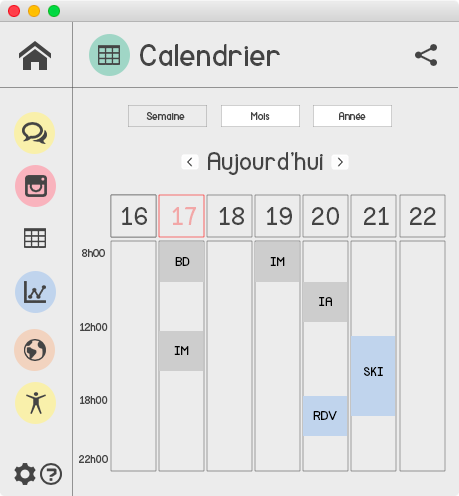
\includegraphics[scale=0.43]{Modelisation/calendrier2.png}
        \caption{Gestion du calendrier}
                \label{fig:calendrier2}
\label{fig:base}
    \end{minipage}\hfill
    \begin{minipage}[b]{0.48\linewidth}
        \centering 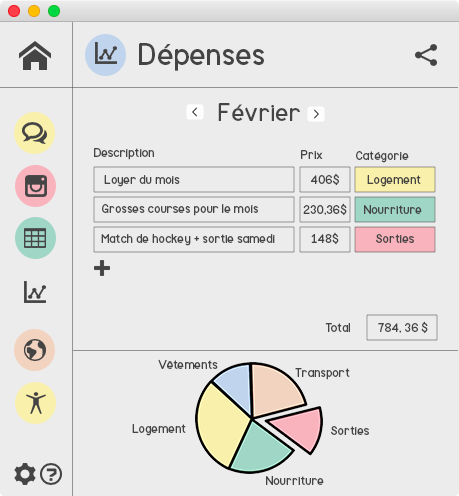
\includegraphics[scale=0.43]{Modelisation/depenses.png}
        \caption{Gestion des dépenses}
         \label{fig:depenses}
    \end{minipage}
\end{figure}
\begin{figure}[hbtp]
    \begin{minipage}[b]{0.4\linewidth}
        \centering 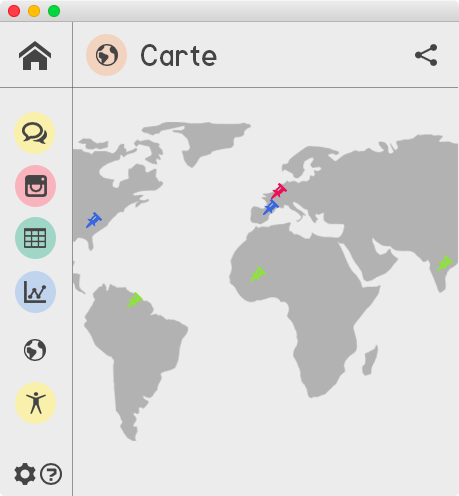
\includegraphics[scale=0.43]{Modelisation/carte.png}
        \caption{Gestion de la carte}
                \label{fig:carte}
\label{fig:base}
    \end{minipage}\hfill
    \begin{minipage}[b]{0.48\linewidth}
        \centering 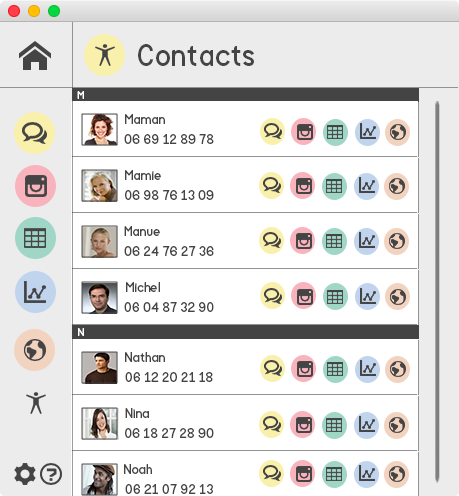
\includegraphics[scale=0.43]{Modelisation/contact.png}
        \caption{Gestion des contacts}
         \label{fig:contact}
    \end{minipage}
\end{figure}

\newpage
\listoffigures


\end{document}